\chapter{The CalTech Continuum Backend (CCB)}\label{chap:ccb}

The Caltech Continuum Backend (CCB) is a dedicated continuum backend
for the GBT Ka-band receiver, built in collaboration with
A.C.S. Readhead's radio astronomy instrumentation group at Caltech and
commissioned on the GBT in 2006. The driving consideration behind its
design is to provide fast electronic beam switching in order to
suppress the electronic gain fluctuations which usually limit the
sensitivity of continuum measurements with single dish radio
receivers. To further improve stability, it is a {\it direct
  detection} system: there are no mixers before the conversion from RF
to detected power. The Ka-band receiver provides {\it eight}
simultaneous, directly detected channels of RF power levels to the
CCB: one for each feed, times four frequency channels ($26$-$29.5$
GHz; $29.5$-$33$ GHz; $33$-$36.5$ GHz; and $36.5$-$40$
GHz). Astronomical information and labels for these 8 channels (or
``ports'' in GBT parlance) is summarized in Table~\ref{tbl:ccbports}.

\begin{table}
\begin{center}
\begin{tabular}{llll}
Port & Beam & Polarization & Frequency \\ \toprule
9 &  1 & Y & $38.25$ \\
10 & 1 & Y & $34.75$ \\
11 & 1 & Y & $31.25$ \\
12 & 1 & Y & $27.75$ \\
13 & 2 & X & $38.25$ \\
14 & 2 & X & $34.75$ \\
15 & 2 & X & $31.25$ \\
16 & 2 & X & $27.75$ \\ \bottomrule
\end{tabular}
\caption[CCB Port labels and the astronomical quantities they measure]
{CCB Port labels and the astronomical quantities they measure.\label{tbl:ccbports}}
\end{center}
\end{table}

The following sections outline the process of observing with, and
analyzing the data from, the CCB. Much of the information in this
chapter is also maintained at 

\noindent
{\tt /users/bmason/ccbPub/README.txt}

\noindent
which is convenient, for instance, for cutting and pasting data analysis commands.
Template scheduling blocks are also in this directory.

%++++++++++++++++++++++++++++++++++++++++++++++++++++++++++++++++++++++++++++
\section{Observing with the CCB}

\subsection{Configuration}

Configuration of the CCB is straightforward, and for most
purposes the only two configurations needed are provided in the two
configuration files 

\noindent
{\tt /users/bmason/ccbPub/ccb.conf} 

\noindent
and 

\noindent
{\tt /users/bmason/ccbPub/ccbBothCalsLong.conf}. 

\noindent
These differ only in the duration of the integrations: the former
configures for 5 millisecond integrations, which is useful for
estimating the scatter in the samples to obtain meaningful $\chi^2$
values in the analysis of science data; the later configures for 25
millisecond integrations, which is useful in peak/focus observations
to speed up processing of the data (see Chapter~\ref{chap:datadisplay}, section~\ref{sec:pointandfocus}). 
{\tt ccb.conf} is reproduced and explained below.

The following keywords tell ASTRID to expect beamswitched continuum
observations with Ka and the CCB:

\begin{lstlisting}[language=PythonAstrid,frame=single,framerule=1pt]
receiver='Rcvr26_40'
beam='B12'
obstype='Continuum'
backend='CCB'
nwin=4
restfreq=27000,32000,35000,38000
deltafreq=0,0,0,0
bandwidth=600,600,600,600
swmode='sp'
swtype='bsw'
pol='Circular'
vdef='Radio'
frame='topo'
\end{lstlisting}

They do not have any practical effect on the actual instrument
configuration but are necessary to set up internal variables and
ensure the recorded FITS files are accurate.

\begin{lstlisting}[language=PythonAstrid,frame=single,framerule=1pt]
ccb.cal_off_integs=20
ccb.XL_on_integs=2
ccb.both_on_integs=2
ccb.YR_on_integs=2
ccb.bswfreq=4
tint=0.005
\end{lstlisting}

\noindent The meaning of these keywords is as follows:
\begin{itemize}
\item The first four specify the cal firing pattern.
\item {\tt ccb.bswfreq} specifies the beam switching frequency in kHz.
4 kHz is standard; the \dq{$> 10\%$ blanking} warning which results is
also standard and may be safely ignored.
\item {\tt tint} is the integration time in seconds.
\end{itemize}

\newpage

\subsection{Pointing \& Focus}

The online processing of pointing and focus data is handled by \gls{GFM}
(which runs within the Astrid Data Display window)
similarly as for other \gls{GBT} receivers and the \gls{DCR}. A few 
comments:
\begin{itemize}
\item because the \gls{Kaband} receiver currently only has one polarization
per beam, \gls{GFM} will by default issue some complaints which can be ignored.
These can be eliminated by choosing \dq{Y/Right} polarization in 
the \gls{Astrid} Data Display window (see Chapter~\ref{chap:datadisplay}, section ~\ref{sec:gfmdataprocessing})
under Tools $\rightarrow$ Options $\rightarrow$ Data Processing.
\item in the same menu ( Tools $\rightarrow$ Options $\rightarrow$ Data Processing),
choosing \dq{31.25 GHz} as the frequency to process, instead of the
default $38.25$ GHz, can improve robustness of the result.
\item The results shown in the Astrid Display are in {\it raw counts}, not Kelvin
or Janskys.
\item Choosing \dq{Relaxed} heuristics is also often helpful.
\end{itemize}

There is a template pointing and focus \gls{SB} for the CCB in 
{\tt /users/bmason/ccbPub} called {\tt ccbPeak.turtle}. This scheduling
block does a focus scan, four peak scans, and a symmetric nod (for
accurate photometry to monitor the telescope gain).


\subsection{Observing Modes \& Scheduling Blocks}

Science projects with the CCB typically fall into two categories:
mapping, and point source photometry.  The majority of CCB science is
the latter, since this is what, by design, it does best. Template
scheduling blocks for both are in {\tt /users/bmason/ccbPub}. 

\begin{center}
\fbox{\parbox{\textwidth}{
{\bf
Observers and support scientists are strongly encouraged to use
these template scheduling blocks as the basis for their CCB
observing scripts and make only the changes that are
required! Relatively innocuous changes can make the data
difficult or impossible to calibrate with existing analysis 
software.}
}}
\end{center}

\noindent The basic template \glspl{SB} are:
\begin{itemize}
\item {\tt ccbObsCycle.turtle}: perform photometry
on a list of sources.
\item {\tt ccbRaLongMap.turtle}: perform a standard {\tt RALongMap} on
a source (see ~\ref{sec:mappingscans}.
\item {\tt ccbMap.turtle, ccbMosaicMap.turtle}: make maps using longer,
single-scan, custom raster maps.  Your staff friend will help tailor
these to your project's needs, should  you choose this approach.
\end{itemize}

Point source photometry is accomplished with an \gls{OTF} variant of
the symmetric NOD procedure described in ~\ref{sec:observingscans}.
This procedure, which we refer to as the
OTF-NOD, alternately places the beam in each of the two beams of the
\gls{Kaband} receiver in a B1/B2/B2/B1 pattern.  This sequence cancels
means and gradients in the atmospheric or receiver emission with time.
Plotting the beamswitched data from this sequence produces a sawtooth
pattern shown in Figure~\ref{fig:otfnodconcept}; this is discussed
more in \S~\ref{sec:onlineanalys}.  Each NOD is 70 seconds long (10
seconds in each phase, with a 10 second slew between beams and an
initial 10 second acquire time).

Note: OTF-NOD is not one of the standard scan types; it is implemented in 
the scripts mentioned here (e.g., \dq{ccbObsCycle.turtle}).

\begin{figure}
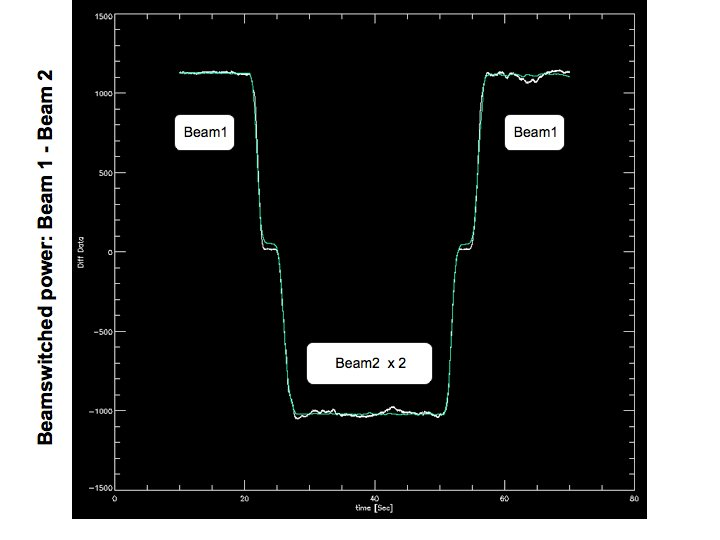
\includegraphics[width=0.7\linewidth]{ccbTutorial23feb09-010.jpg}
\caption[Data from a CCB, beamswitched OTF-NOD]
{Data from a CCB, beamswitched OTF-NOD, showing data and model
versus time through one B1/B2/B2/B1 scan. The white line is the CCB
beamswitched data and the green line is the fit for source amplitude
using the known source and telescope (as a function of time)
positions.}
\label{fig:otfnodconcept}
\end{figure}


\subsection{Calibration}

If at all possible, be sure to do a peak and focus, and perform
photometry (an OTF-NOD, as implemented in {\tt ccbObsCycle.turtle} or
{\tt ccbPeak.turtle}) on one of the following three primary (flux)
calibrators: 3c48, 3c147, or 3c286. This will allow your data to be
accurately calibrated (our calibration scale is ultimately referenced
to the WMAP 30 GHz measurements of the planets). If this is not
possible the calibration can be transferred from another telescope
period (observing session) within a few days of the session in
question.

\subsection{Online Data Analysis}
\label{sec:onlineanalys}

It is important to assess data quality during your observing session.
There are a set of custom IDL routines for analyzing CCB data; if you
use the observing procedures and config files described here, your
data should be readily calibratable and analyzable by them. To
use the IDL code, start IDL by typing (from the GB UNIX command line)
\begin{lstlisting}
/users/bmason/ccbPub/ccbidl
\end{lstlisting}

Here is an example data reduction session that provides a quick look at your data:

\begin{lstlisting}
; set up global variables
;  don't write files or plots to disk...
proj='AGBT06A_049_09'
setccbpipeopts,gbtproj=proj,ccbwritefiles=0,\$
  gbtdatapath='/home/archive/science-data/tape-0016/'
; to use postprocessing scripts, set ccbwritefiles=1

; a good color table for the plots:
loadct,12

; create an array indexing scan numbers
;  to file name
indexscans,si

; summarize the project
summarizeproject

; read a nod observation from scan 12
readccbotfnod,si[12],q
; fit the data, binning integrations to 0.5sec bins
fitccbotfnod,q,qfit,bin=0.5
; the resulting plot shows the differenced
;  data (white) and the fit to the data (green)
;  for each of 16 CCB ports. (the first 8 are blank)

; look at the next nod that just came in
;  this time calibrate to antenna temperature
;  before plotting
; First you need to derive a calibration, which
;  requires a scan with both cals firing independently.
; /dogain tells the code to solve for the calibration;
;  the results are stored in calibdat, which we can
;  pass into subsequent invocations of the calibration.
indexscans,si
readccbotfnod,si[13],q
calibtokelvin,q,/dogain,calibdat=calibdat
fitccbotfnod,q

; the scan index si must be updated to read in scans
;  collected after it was first created
indexscans,si
readccbotfnod,si[14],q
; and calibrate to kelvin using the information
;  we just derived
calibtokelvin,q,calibdat=calibdat
; fit/plot
fitccbotfnod,q

; et cetera...

\end{lstlisting}

Example OTF-NOD data for bright sources (under good and poor
conditions) and a weak source (under good conditions)
are shown in Figures~\ref{fig:brightgood} through
\ref{fig:weakbinned}

\begin{figure}
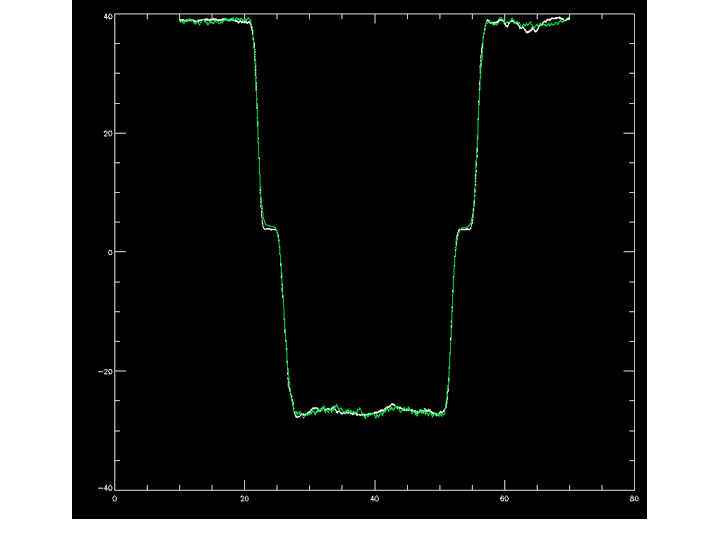
\includegraphics[width=4.5in,bb=0 0 720 540]{ccbTutorial23feb09-011.png}
\caption[CCB data from an OTF-NOD observation of a bright source]
{CCB data from an OTF-NOD observation of a bright source, showing data and model
versus time through one B1/B2/B2/B1 scan. The white line is the CCB
beamswitched data and the green line is the fit for source amplitude
using the known source and telescope (as a function of time)
positions. The close agreement between the data and the fit indicate
that neither fluctuations in atmospheric emission nor pointing
fluctuations (typically due to the wind on these timescales) are
problems in this data.}
\label{fig:brightgood}
\end{figure}


\begin{figure}
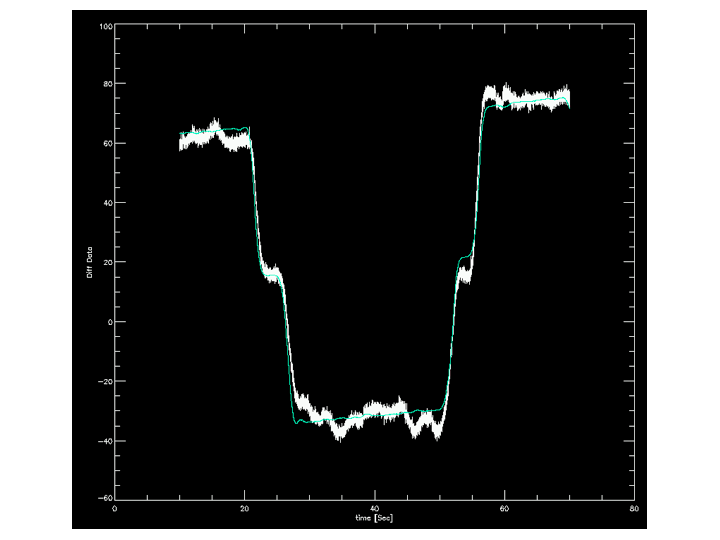
\includegraphics[width=4.5in,bb=0 0 720 540]{ccbTutorial23feb09-012.png}
\caption[CCB OTF-NOD data on a bright source under marginal conditions]
{CCB OTF-NOD data on a bright source under marginal conditions.The
differences between the data and the model are clearly larger in this case.}
\label{fig:brightpoor}
\end{figure}


\begin{figure}
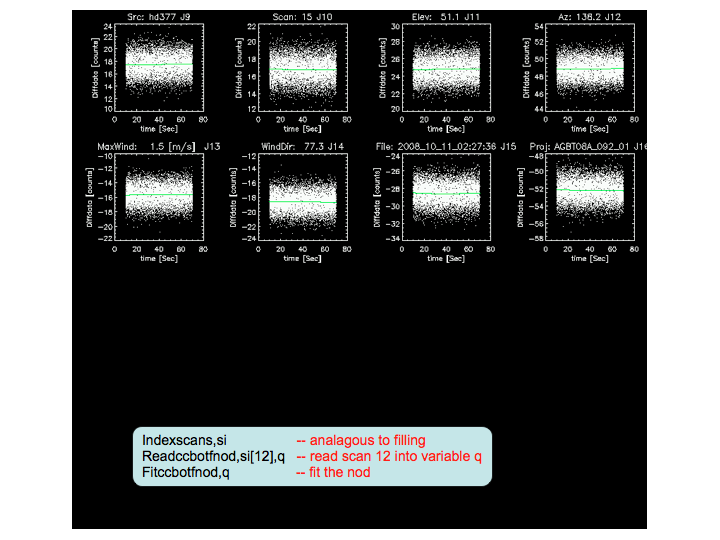
\includegraphics[width=4.5in,bb=0 0 720 540]{ccbTutorial23feb09-013.png}
\caption[CCB OTF-NOD measurement of a weak (mJy-level) source under good conditions]
{CCB OTF-NOD measurement of a weak (mJy-level) source under good conditions. The
IDL commands used to obtain this plot are shown inset.}
\label{fig:weak}
\end{figure}


\begin{figure}
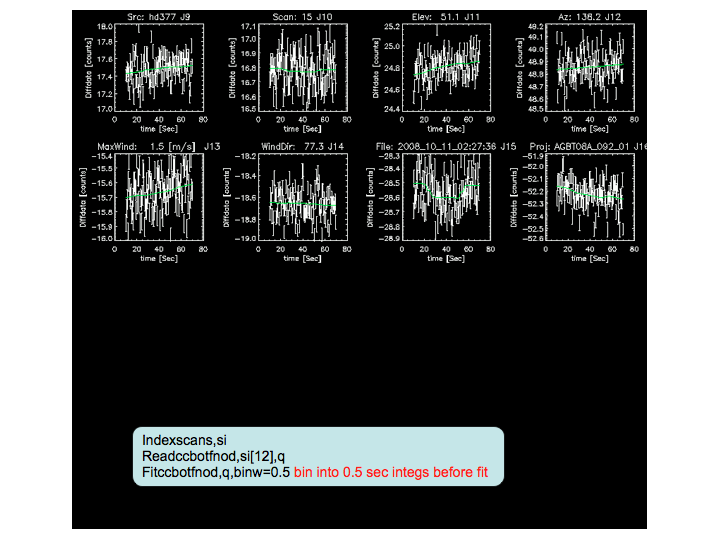
\includegraphics[width=4.5in,bb=0 0 720 540]{ccbTutorial23feb09-014.png}
\caption[The same weak-source data with the individual integrations
binned into $0.5$ second bins]
{The same weak-source data, this time with the individual integrations
binned into $0.5$ second bins (using {\tt fitccbotfnod}'s {\tt
binwidth} optional argument in seconds) so the thermal-noise scatter
doesn't dominate the automatically chosen $y$-axis scale. This better
shows any gradients or low-level fluctutions in the beamswitched data
(due, for instance, to imperfect photometric conditions). In this data
they are not significant.}
\label{fig:weakbinned}
\end{figure}


Mapping data can also be imaged using the IDL tools:
\begin{lstlisting}
; make a map from scans 7-10 using port 11 data 
;  (note the port must be specified; valid ports are
;   9-16)
img=makedcrccbmap([7,8,9,10],/isccb,port=11)
; replot the map
plotmap,img,/int
; make a png copy of it
grabpng,'mymap.png'
; save the map in standard FITS format--
saveimg,img,'mymap.fits'
\end{lstlisting}
This will be a {\it beamswitched} map. The beamswitching can be
removed by an EKH\footnote{Emerson, Klein, Haslam 1979 A\&A {\bf 76},92.} 
deconvolution algorithm also implemented in the
code. Your GBT friend will help you with this, if needed.

\section{Performance}

Recent tests under excellent conditions show a sensitivity of $150
\, \mu {\rm Jy}$ (RMS) for the most sensitive single channel (34 GHz),
or $100 \, \mu {\rm Jy}$ (RMS) for all channels combined
together. These are the RMS of fully-calibrated, 70-second OTF-NODs on
a very weak source.  Typical ``reasonable-weather'' conditions are a
factor of two worse.  Improvements to the receiver made since these
data were acquired may result in better sensitivity for the 2010/2011
season.

\section{Differences Between the CCB/Ka System and other GBT Systems}

There are a few differences between the CCB/Ka system and other GBT
receiver/backend systems which users familiar with the GBT will want
to bear in mind.
\begin{itemize}

\item Because it is a direct detection system, the GBT IF system does not enter into observing. 

\item The Ka/CCB gains are engineered to be stable (10\% - 20\% over months), so no variable attenuators are in the signal
chain. Consequently there is no {\tt Balance()} step.

\item To optimize the RF balance (for spectral baseline and continuum stability), the OMT's have been
removed from the Ka band receiver. It is therefore sensitive to {\it
one linear polarization per feed}.  The two feeds are sensitive to
orthogonal linear polarizations (X and Y).

\item Feed orientation is $45^\circ$ from the Elevation/cross-Elevation axes.
All other receivers have feed separations that are parallel to the Elevation
or cross-Elevation axes (except for the \gls{KFPA}).

\item There are two cal diodes (one for each feed), and they are separately controlled ({\it i.e.}, it is
possible to turn one on and not the other). Cals are ON or OFF for an
entire integration; they are not pulsed ON and OFF within a single
integration.

\end{itemize}



